\section{Предметная область}
\label{subject_area} \index{Chapter2}

Введем определения, используемые в данной работе:


\begin{table}[ht]
\centering
\caption{Нотация}
\fontsize{12}{14}\selectfont
\renewcommand{\arraystretch}{1.2} % Увеличиваем высоту строк
\begin{tabularx}{\textwidth}{>{\centering\arraybackslash}m{3cm} >{\centering\arraybackslash}m{3cm} >{\centering\arraybackslash}X}
\toprule
\textbf{Термин} & \textbf{Обозначение} & \textbf{Описание} \\
\midrule
Корпус документов & $\mathcal D = \{d_i\}_{i=1}^{|\mathcal D|}$ & Множество объектов, где $d_i$ — фрагмент документации после этапа предобработки. \\
\midrule
Retriever & $f_{\phi}, f_{\psi}$ & Отображения текстовых данных в $\mathbb{R}^m$ с параметрами $\phi$ и $\psi$. Отображение $f_{\phi}$ для пользовательских запросов, а $f_{\psi}$ для документов.\\
\midrule
Метрика близости & $Sim(q,d)$ & Семантическая близость между запросом и документом. \\
\midrule
Generator (LLM) & $g_\theta$ & Отображение, параметризованное $\theta$. \\
\midrule
Запрос & $q$ & Пользовательский запрос. \\
\midrule
Контекст & $c$ & Контекст запроса. \\
\midrule
Ответ & $a$ & Целевой ответ. \\
\midrule
QA датасет & $X = \{X_i\}_{i=1}^{|X|}$ & Набор объектов, где $X_i$ = $(q_i, c_i, y_i)$. \\
\bottomrule
\end{tabularx}
\end{table}


Обучением модели будем называть процесс построения оптимального отображения, минимизирующего целевую функцию потерь.

Обучаемыми параметрами модели - параметры отображения, которые могут изменяться в ходе процесса обучения модели для получения оптимального результата.

\subsection{Большая языковая модель}
\label{subsec:math} \index{Chapter2!Math}

С точки зрения формальной математической постановки большая языковая модель это отображение, моделирующее вероятностное распределение следующего токена (символа или части слова) в текста, т.е. $g_\theta: \mathcal V^{\!*} \mapsto [0, 1]^{|\mathcal V|}$, где $\mathcal V$ фиксированный словарь.

Вероятность последовательности токенов $(x_1, \ldots, x_{T})$ факторизуется авторегрессионно:

\begin{equation}
    P_{\theta}(x_1, \ldots, x_{T}) = \prod_{t=1}^{T} P_{\theta}(x_t \mid x_{<t}) \textit{, где $g_{\theta}(x_{\leq t}) = P_{\theta}(\cdot \mid x_{\leq t})$}
\end{equation}

Обучение производится на большом корпусе $D = \{(x_1^{(i)}, \ldots, x_{T_i}^{(i)}\}_{i=1}^{N}$ через вычисление оценки максимального правдоподобия, путем минимизации среднего отрицательного логарифма правдоподобия (NLL loss):

\begin{equation}
    \mathcal{L}_{LM}(\theta) = - \frac{1}{N} \sum_{i=1}^N \sum_{t=1}^{T_i} log P_{\theta}(x_t^{(i)} \mid x_{<t}^{(i)})
    \label{generative_loss}
\end{equation}

Этот этап обычно называют предварительным обучением (pretrain). На нём модель <<получает>> основные знания о мире и оптимизируется для правдоподобного продолжения текстов. 

Следующим этапом является обучение на датасетах, составленных из инструкционных пар $D = \{I^{(i)}, R^{(i)}\}_{i=1}^{N} \textit{, где}$ 

\begin{itemize}
    \item $I^{(i)} = (l_1^{(i)}, \ldots, l_{L_i}^{(i)})$ - описание задачи на естественном языке.

    \item $R^{(i)} = (r_1^{(i)}, \ldots, r_{T_i}^{(i)})$ - ожидаемый ответ.
\end{itemize}

В данном случае задачей для LLM ставится генерация R. В частности функция потерь приобретает вид:

\begin{equation}
    \mathcal{L}_{SFT}(\theta) = - \frac{1}{N} \sum_{i=1}^N \sum_{t=1}^{T_i} log P_{\theta}(r_t^{(i)} \mid l_1^{(i)}, \ldots, l_{L_i}^{(i)} ,r_{<t}^{(i)})
\end{equation}

Этот этап называется Instruct Tuning или же Supervised Finetuning (SFT). Он необходим для адаптации модели к выполнению запросов, описанных на ествественном языке.  

Частным случаем инструкционного обучения является question-answering на датасете X:

\begin{equation}
    \mathcal{L}_{QA}(\theta) = - \frac{1}{|X|} \sum_{i=1}^X \sum_{t=1}^{T_i} log P_{\theta}(a_t^{(i)} \mid q^{(i)}, c^{(i)} ,a_{<t}^{(i)})
\end{equation}


\subsection{Retriever и генерация в RAG}
\label{subsec:rag} \index{Chapter2!RAG}

Как упоминалось ранее, в архитектуре RAG за создание информативных векторных представлений отвечает отдельный Retriever модуль. Формально, он задается как отображение $f: \mathcal T \mapsto \mathbb{R}^m$, где $\mathcal T$ - пространство текстов. Такие модели также называют эмбеддерами(embedder), а создаваемые ими представления эмбеддингами (embedding), они играют важную роль во множества задач машинного обучения. Ключевым требованием для информативности является:

\begin{itemize}
    \item $f(x) \approx f(y)$, если тексты $x$ и $y$ схожи по смыслу.
    \item $f(x) \not\approx f(y)$, если тексты $x$ и $y$ различны по смыслу.
\end{itemize}

Cемантическую близость полученных векторов чаще всего вычисляется по формуле косинусной меры близости или скалярного произведения:
\begin{equation}
   Similarity(q, d_i) = \langle f_{\phi}(q) \; , \; f_{\psi}(d_i) \rangle = f_{\phi}(q)^{\top} f_{\psi}(d_i)
\end{equation}

Принцип работы изображен на рис. \ref{retrieval}.

\begin{figure}[h!]
    \centering
    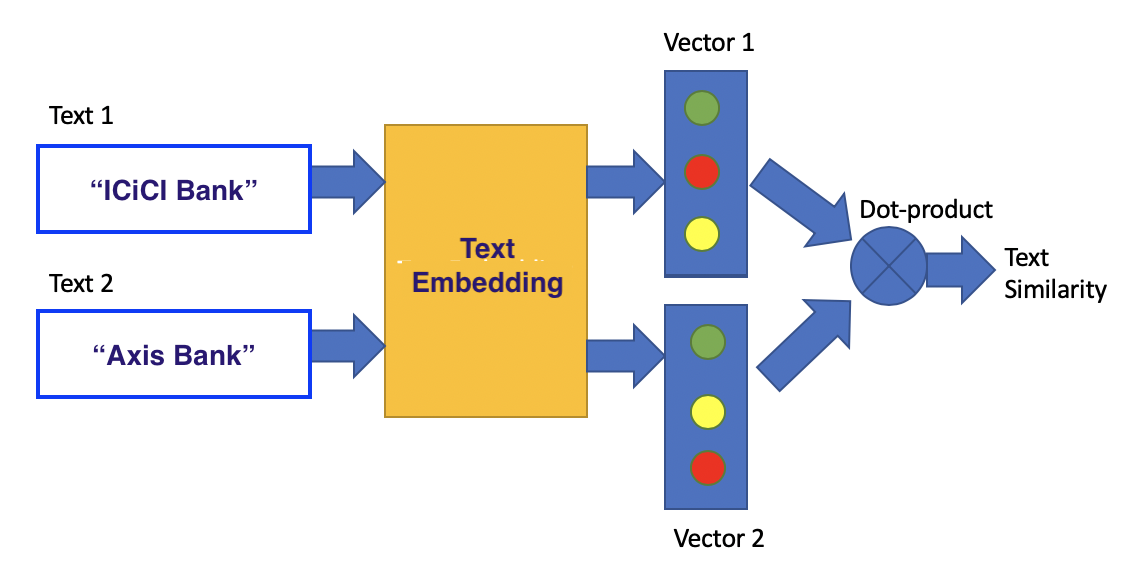
\includegraphics[scale=0.8]{./images/embedder.png}
    \caption{\protect\hypertarget{image1}{Алгоритм поиска метрики близости.}}
    \label{retrieval}
\end{figure}

Обучение retriever модели как правило основано на contrastive learning, когда для каждого запроса $q$ есть разметка, состоящая из целевого документа $d^{+}$ и набора нерелевантных документов $d^{-} = (d_1^{-}, \ldots, d_l^{-})$, а задачей является увеличение близости векторных представлений для $q$ и $d^{+}$, одновременно с уменьшением для $q$ и $d^{-}$.

Тогда вероятность релевантности документа $d \in \mathcal D$ к запросу $q$ оценивается как: 

\begin{equation}
    P(d \mid q) = \frac{exp(\langle f_{\phi}(q) \; , \; f_{\psi}(d) \rangle)}{\sum_{d' \in D}exp(\langle f_{\phi}(q) \; , \; f_{\psi}(d') \rangle)}
\end{equation}

А функция потерь на 1 объекте имеет вид:

\begin{equation}
    \mathcal{L}_{Retrieval} = -log P(d^{+} \mid q) = - log \frac{exp(\langle f_{\phi}(q) \; , \; f_{\psi}(d^{+}) \rangle)}{\sum_{d' \in D}exp(\langle f_{\phi}(q) \; , \; f_{\psi}(d') \rangle)}
    \label{retrieval_loss}
\end{equation}

При последующей генерации ответов языковая модель использует несколько наиболее вероятных документов. Другими словами, в качестве контекста для генерации LLM используются top-K фрагментов с наибольшей метрикой близости к запросу:

\begin{equation}
   c = \argmax_{\{{d_i}\}_{i=1}^K} \sum_{i=1}^K Similarity(q, d_i).
\end{equation}

\subsection{Архитектуры моделей}
\label{subsec:language_model} \index{Chapter2!Language model}


% Такая архитектура способна замечать более тонкие смысловые связи между запросом и документом, что зачастую повышает качество поиска. Однако, в то же время, нельзя гарантировать полную релевантность найденных документов.

В задачах Natural Language Processing (NLP) большое распространение получили трансформерные архитектуры, представленные в работы <<Attention Is All You Need>> \cite{transformer} (рис. \ref{transformer}).

\begin{figure}[ht!]
    \centering
    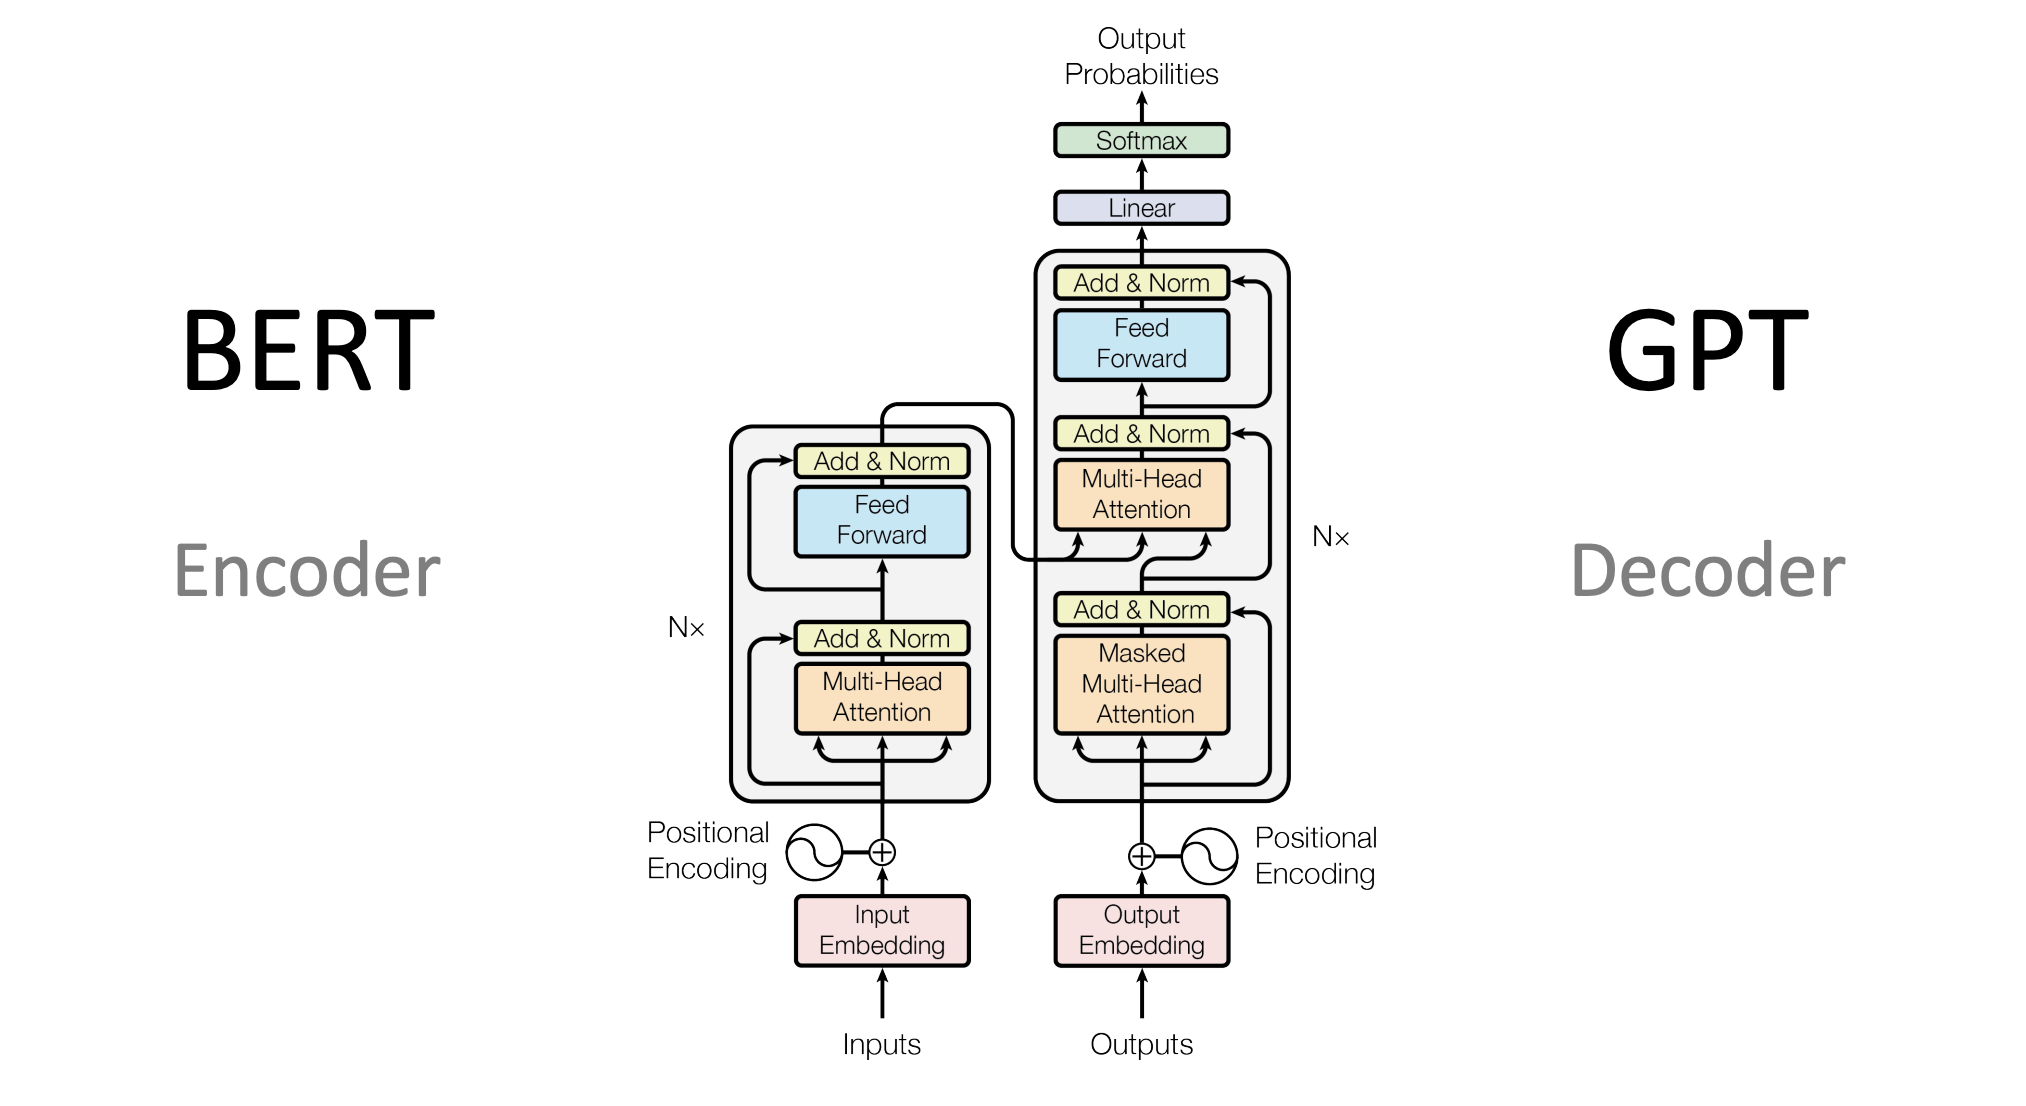
\includegraphics[scale=0.45]{images/transformers.png}
    \caption{Encoder-Decoder архитектура трансформер, оригинальное изображение взято из \cite{transformer}.}
    \label{transformer}
\end{figure}

Ключевой особенностью оригинальной архитектуры является представление в виде encoder-decoder пары, а также добавление механизма внимания, который учитывает влияние каждого элемента последовательности на текущий. Формально, self-attention вычисляется следующим образом:
\begin{equation}
    Attention(Q, K, V) = softmax(\frac{Q K^{\top}}{\sqrt{d_k}})V
\end{equation}
где $Q, K, V$ -- это матрицы запросов (queries), ключей (keys) и значений (values) соответственно, а $d_k$ -- размерность векторного пространства представлений.

Механизм внимания позволяет модели эффективно обрабатывать длинные текстовые последовательности ценой большей вычислительной сложности. Данная работа ограничивается рассмотрением только трансформерных архитектур. 

Дальнейшие исследования показали, что для генеративных задач наибольшую эффективность показывают gpt-подобные decoder-only архитектуры, обученные на кросс-энтропийной функции потерь (\ref{generative_loss}). 

Для embedder модели чаще всего применяются bert-подобные encoder-only архитектуры, обученные на контрастивную функцию потерь (\ref{retrieval_loss}).


% В частности, будем использовать открытые предобученные инструкционные модели. После этапа языкового моделирования на большом объеме данных они дополнительно обучаются на задачах, требующих следовать определенным инструкциям. Это необходимо для адаптации модели к формату вопрос-ответ, а также улучшению качества генерации при специализированном запросе.



\subsection{Метод Low-Rank Adaptation (LoRA)}
\label{subsec:lora} \index{Chapter2!LoRA}

Для эффективной адаптации языковой модели к целевой задаче в условиях ограничения вычислительных ресурсов чаще всего применяется метод низкоранговой адаптации \cite{LoRA}. Идея заключается в обновление исходных параметров $\mathbf{W}$ путём их заморозки и добавления $\Delta \mathbf{W}$, состоящего из низкорангового разложения (рис. \ref{lora}):

\begin{equation}
    \Delta \mathbf{W} = \mathbf{B}\mathbf{A}, \textit{где:}
\end{equation}

\begin{itemize}
    \item $\Delta \mathbf{W} \in R^{d \times k}$ -- матрица адаптации того же размера, что и исходная замороженная матрица весов $\mathbf{W}$.
    \item $\mathbf{B} \in \mathbb{R}^{d \times r}$, $\mathbf{A} \in \mathbb{R}^{r \times k}$ -- обучаемые матрицы.
    \item $r \ll \min(d, k)$ -- ранг разложения.
\end{itemize}

\begin{figure}[ht!]
    \centering
    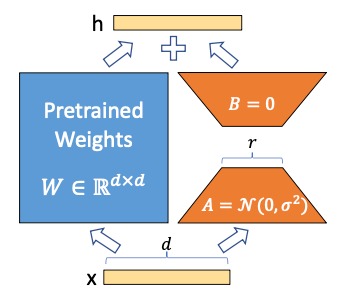
\includegraphics[scale=0.65]{images/lora_good.png}
    \caption{LoRA адаптер, изображение из \cite{LoRA}.}
    \label{lora}
\end{figure}

\noindentИтоговый слой модели действует следующим образом:
\begin{equation}
    W'(x) = h = \mathbf{W}x + \frac{\alpha}{r} \mathbf{B}\mathbf{A}x, \text{где $\alpha$ это гиперпараметр масштабирования.}
\end{equation}


\noindentИнициализация параметров:
\begin{itemize}
    \item $\mathbf{A} \sim \mathcal{N}(0, \sigma^2).$
    \item $\mathbf{B} = \mathbf{0}$ (нулевая инициализация).
\end{itemize}



\noindentСреди преимуществ метода можно выделить
\begin{itemize}
    \item Параметрическая эффективность (обучения 0.5-2\% от размера исходных параметров).
    \item Снижение риска катастрофического забывания.
    \item Высокая скорость обучения.
\end{itemize}



\subsection{Методы оценки качества}
\label{subsec:scoring_theory} \index{Chapter2!Scoring theory}

\subsubsection{ROUGE}
\label{subsec:rouge} \index{Chapter6!rouge}

ROUGE (Recall-Oriented Understudy for Gisting Evaluation) - серия метрик, предложенная в работе <<ROUGE: A Package for Automatic Evaluation of Summaries>> \cite{ROUGE} для оценки качества решения задачи суммаризации текста. 

Пусть есть 2 текста - сгенерированный $G$ и целевой $R$. Разобъем их на униграммы (отдельные слова), тогда определены следующие метрики:

\begin{equation}
    \textit{ROUGE-1 Precision} = \frac{\textit{Количество совпадающих униграм в $G$ и $R$}}{\textit{Количество униграм в G}}
\end{equation}

\begin{equation}
    \textit{ROUGE-1 Recall} = \frac{\textit{Количество совпадающих униграм в $G$ и $R$}}{\textit{Количество униграм в R}}
\end{equation}

\begin{equation}
    \textit{ROUGE-1 F1-score} = 2\frac{\textit{precision $\cdot$ recall}}{\textit{precision + recall}}
\end{equation}

Аналогично определяются метрики ROUGE-N, путём разбиения текста на $n$-граммы. Метрики ROUGE-L определены с использованием longest common subsequence (LCS):

\begin{equation}
    \textit{ROUGE-L Precision} = \frac{\textit{LCS($G$, $R$)}}{\textit{Количество униграм в G}}
\end{equation}

\begin{equation}
    \textit{ROUGE-L Recall} = \frac{\textit{LCS($G$, $R$)}}{\textit{Количество униграм в R}}
\end{equation}

Важно отметить, что подобные метрики не могут в полной мере оценить качество, так как являются чувствительными к порядку слов и использованию синонимов.


\subsubsection{LLM как судья}
\label{subsec:llm_judge} \index{Chapter6!llm_judge}

Еще одним стандартным подходом для оценки качества суммаризации является использование нейросетевых методов. В частности метод LLM-as-judge предполагает использование генеративных языковых моделей для имитации человеческой оценки.

Множество исследований показывают (\cite{LLM-as-judge-1}, \cite{LLM-as-judge-2}, \cite{LLM-as-judge-3}), что хотя использование LLM для оценки качества на данный момент не может в полной заменить человеческую оценка, однако между ними уже сейчас имеется согласованность порядка 80\% \cite{LLM-as-judge-1}.  

В данной работе в качестве модели-судьи будет выступать Llama-3.3-70B-Instruct. На вход модели подается вопрос пользователя, релевантный фрагмент текста, эталонный ответ, сгенерированный ответ и подробная инструкцию по оценке. Запрос можно найти в приложении A \ref{app:judge_prompt}.

\subsection{Бенчмарк}
\label{subsec:benchmark_theory} \index{Chapter2!Benchmark theory}

Для оценки качества RAG-системы нужна специализированная процедура. На текущий момент в открытом доступе отсутствуют русскоязычные бенчмарки, в полной мере отвечающие всем требованиям. Во многом это обусловлено отсутствием стандартизированных метрик качества контекстно-зависимой QA генерации. Классические статистические методы не подходят для всесторонней оценки реального качества, а крупные коммерческие компании чаще всего используют дорогостоящую человеческую разметку. В связи с этим актуальной становится задача создания бенчмарка,  максимально приближенного к практическим сценариям применения RAG.

В качестве доменов для бенчмарка были выбраны 3 следующие сферы: Статьи и регламенты, техническая документация, финансовые отчеты. Для эффективной работы в этих областях требуется постоянное взаимодействие с большим количеством текстовой документации. Потому в этом сценарии часто внедряются интеллектуальные ассистенты для оптимизации времени поиска нужной информации.

Однако при оценка важно учитывать не только покрываемые сферы, но также и наиболее частные сценарии применения. По этой причине бенчмарк разделен на несколько типов вопросов, каждый из которых оценивает разные компетентности модели.

Представлены следующие типы вопросов:

\begin{enumerate}
    \item \textbf{\textit{Simple}} - прямые вопросы, требующие нахождения одного фрагмента документации. Оценивают качество работы модели в стандартном сценарии применения.

    \item \textbf{\textit{With errors}} - вопросы, содержащие ряд грамматических и синтаксических ошибок. Требует от модели навыков понимания низкокачественных запросов.

    \item \textbf{\textit{Trash}} - избыточные запросы, содержащие помимо непосредственного вопроса множество текста на отвлеченную тему. Требует от модели навыков понимания запроса в условиях шума.

    \item \textbf{\textit{Reformulation}} - запросы, аналогичные \textit{Simple}, однако переформулированные на более технический стиль или составленные с использованием слов, не содержащихся в текстовом фрагменте, содержащем ответ на вопрос. Требует понимания синонимов или экспертизы в предметной области.

    \item \textbf{\textit{Incorrect by design}} - вопросы, содержащие неверное предположение, провоцирующее на простой, однако неверный ответ. Требует умения не обосновываться на неверный контекст.

    \item \textbf{\textit{Table}} - запросы, требующие извлечения информации из табличных данных. Оценивает навыки работы со структурированными данными.

    \item \textbf{\textit{No info}} - вопросы, ответов на которых нет в документационном индексе. Проверяет навык модели, не придумывать ответ, а явно отвечать, что его нет.

    \item \textbf{\textit{Double}} - запросы, содержащие 2 независимых вопроса одновременно. Оценивает качество работы с разрозненной информацией.

    \item \textbf{\textit{Multi block}} - вопросы, для ответа на которые требуется использование информации из разных фрагментов текстовой документации. Проверяет навык суммаризации информации из разных источников.

    \item \textbf{\textit{Logical thinking}} - вопросы, требующие рассуждений по аналогии или по принципу перехода от <<общего к частному>>. Требует от модели понимания мира и предметной области. 
    
\end{enumerate}

Каждый домен разделен на 3 сета:

\begin{itemize}

    \item \textit{Статьи и регламенты}: медицинские научные статьи (pubmed), регламенты нефтегазовой отрасли, регламенты металлургии.
    
    \item \textit{Техническая документация}: документация linux, инструкции по эсксплуатации техники, руководства к ПО.
    
    \item \textit{Финансовые отчеты}: финансовые отчеты кампаний, аналитические отчеты, отчеты об AI отрасли.
    
\end{itemize}


Поиск документов проводился вручную. Вопросы формировались полуавтоматически с последующей верификацией. Итоговый общий размер - 644 примера (рис. \ref{Benchmark example}). Более детально процесс построения будет описан в практической части работы.

\begin{figure}[ht!]
    \centering
    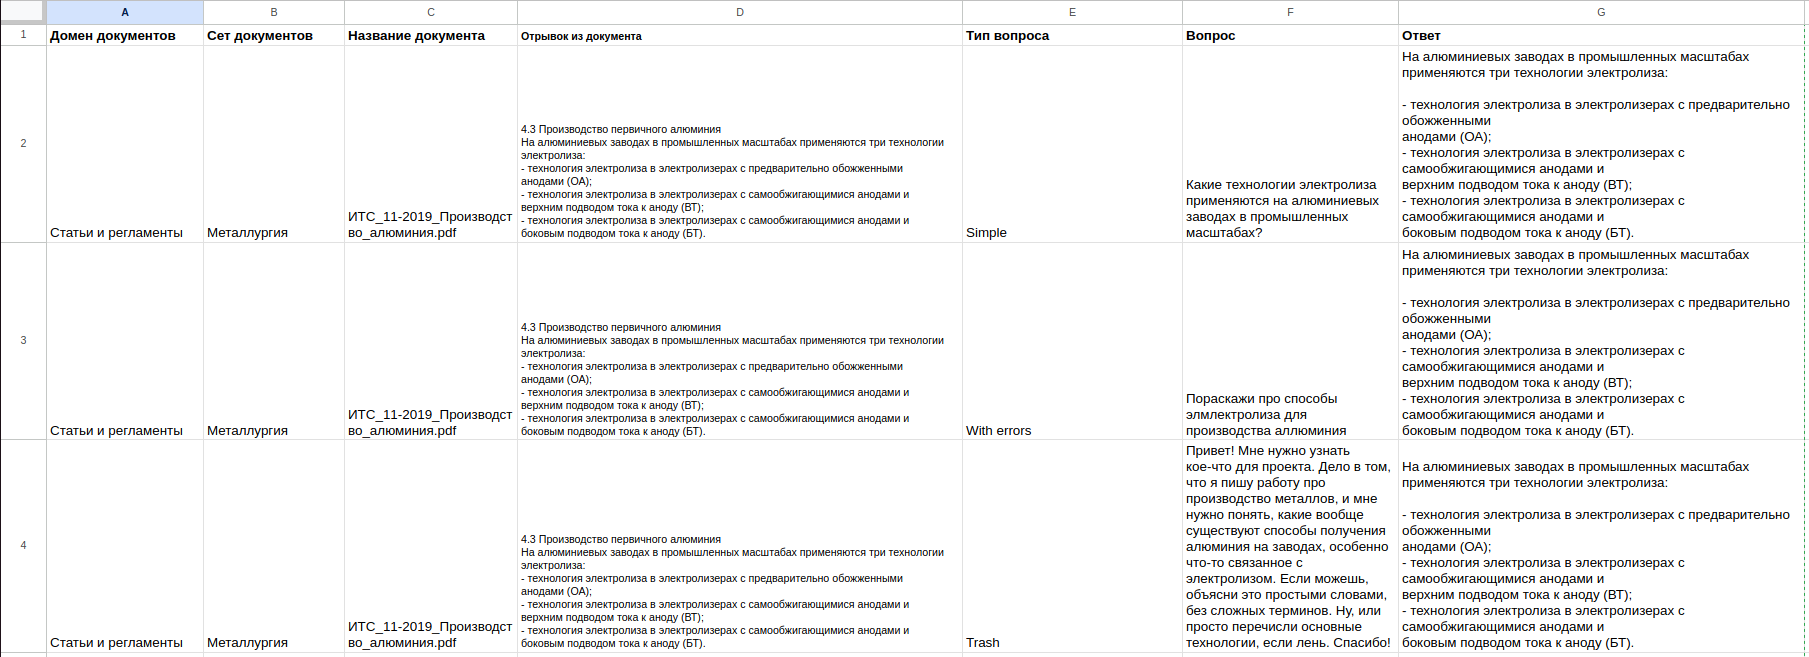
\includegraphics[scale=0.25]{images/Benchmark_data_example.png}
    \caption{Пример данных в бенчмарке.}
    \label{Benchmark example}
\end{figure}

\newpage